\section{Decode Module}

\begin{figure}[h!]
    \centering
    \vspace{1em}
\scalebox{0.85}{
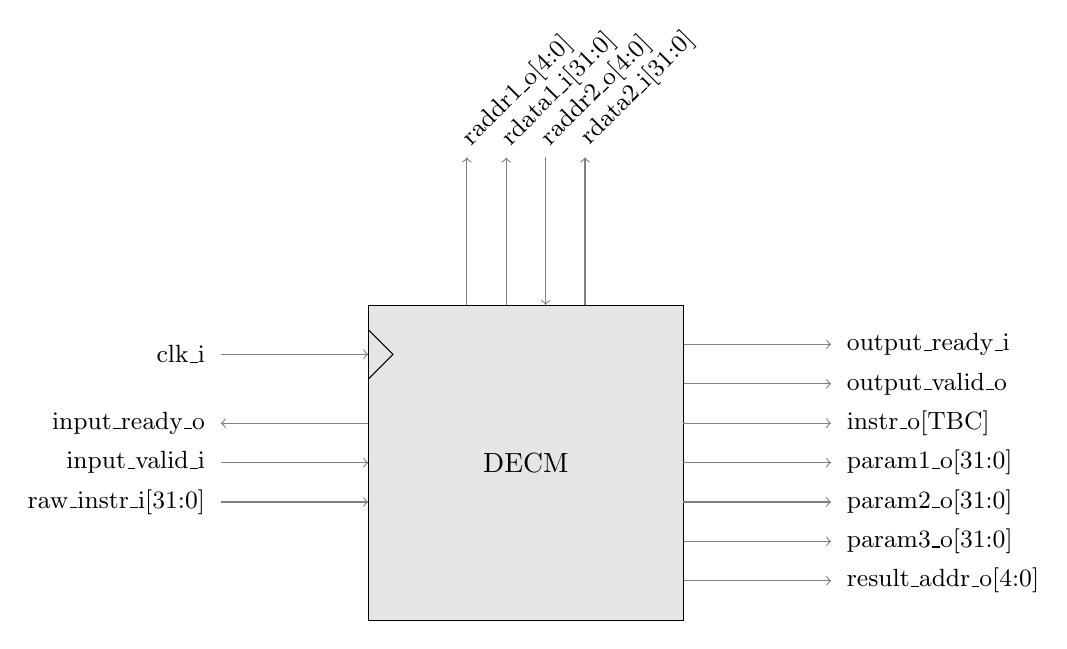
\begin{tikzpicture}[scale=1.25, draw=gray, inner sep=0, outer sep=0]
  \node[rectangle, draw=black,
    anchor=south,
    align=center,
    minimum height = 4cm,
    minimum width = 4cm,
    fill = gray!20] (block) at (0, 0) {DECM};

  \node (rport4) at (block.east) {};
  \node (rport3) at ([yshift=0.4cm]rport4.center) {};
  \node (rport2) at ([yshift=0.4cm]rport3.center) {};
  \node (rport1) at ([yshift=0.4cm]rport2.center) {};
  \node (rport5) at ([yshift=-0.4cm]rport4.center) {};
  \node (rport6) at ([yshift=-0.4cm]rport5.center) {};
  \node (rport7) at ([yshift=-0.4cm]rport6.center) {};
  \draw[<-] ([xshift=1.5cm]rport1.center) node[right=0.2cm, anchor=west]{\small output\_ready\_i} -- (rport1.center);
  \draw[<-] ([xshift=1.5cm]rport2.center) node[right=0.2cm, anchor=west]{\small output\_valid\_o} -- (rport2.center);
  \draw[<-] ([xshift=1.5cm]rport3.center) node[right=0.2cm, anchor=west]{\small instr\_o[TBC]} -- (rport3.center);
  \draw[<-] ([xshift=1.5cm]rport4.center) node[right=0.2cm, anchor=west]{\small param1\_o[31:0]} -- (rport4.center);
  \draw[<-] ([xshift=1.5cm]rport5.center) node[right=0.2cm, anchor=west]{\small param2\_o[31:0]} -- (rport5.center);
  \draw[<-] ([xshift=1.5cm]rport6.center) node[right=0.2cm, anchor=west]{\small param3\_o[31:0]} -- (rport6.center);
  \draw[<-] ([xshift=1.5cm]rport7.center) node[right=0.2cm, anchor=west]{\small result\_addr\_o[4:0]} -- (rport7.center);

  \node(uport2) at ([xshift=-0.2cm]block.north) {};
  \node(uport1) at ([xshift=-0.4cm]uport2.center) {};
  \node(uport3) at ([xshift=0.4cm]uport2.center) {};
  \node(uport4) at ([xshift=0.4cm]uport3.center) {};
  \draw[<-] ([yshift=1.5cm]uport1.center) node[above=0.2cm, anchor=west, rotate=45]{\small raddr1\_o[4:0]} -- (uport1.center);
  \draw[<-] ([yshift=1.5cm]uport2.center) node[above=0.2cm, anchor=west, rotate=45]{\small rdata1\_i[31:0]} -- (uport2.center);
  \draw[->] ([yshift=1.5cm]uport3.center) node[above=0.2cm, anchor=west, rotate=45]{\small raddr2\_o[4:0]} -- (uport3.center);
  \draw[<-] ([yshift=1.5cm]uport4.center) node[above=0.2cm, anchor=west, rotate=45]{\small rdata2\_i[31:0]} -- (uport4.center);

  \node (lport2) at (block.west) {};
  \node (lport1) at ([yshift=0.4cm]lport2.center) {};
  \node (lport3) at ([yshift=-0.4cm]lport2.center) {};

  \draw[<-] ([xshift=-1.5cm]lport1.center) node[left=0.2cm, anchor=east]{\small input\_ready\_o} -- (lport1.center);
  \draw[->] ([xshift=-1.5cm]lport2.center) node[left=0.2cm, anchor=east]{\small input\_valid\_i} -- (lport2.center);
  \draw[->] ([xshift=-1.5cm]lport3.center) node[left=0.2cm, anchor=east]{\small raw\_instr\_i[31:0]} -- (lport3.center);

  \node (clk) at ([yshift=-0.5cm]block.north west) {};
  \draw[->] ([xshift=-1.5cm]lport3.center |- clk.center) node[left=0.2cm, anchor=east]{\small clk\_i} -- (clk.center);
  % clk triangle
  \draw[-  , draw=black] ([yshift=0.25cm]clk.center) -- ([xshift=0.25cm]clk.center) -- ([yshift=-0.25cm]clk.center);
\end{tikzpicture}
}

    \caption{Schematic view of the Decode Module}
    \label{fig:decm}
\end{figure}

\subsection{Interface}

\begin{content}
The decode module implements TBC. The signals are described in table \ref{tab:decm-interface}. 
\end{content}

{
  \vspace{0.5em}
  \begin{center}
    \refstepcounter{table}
    Table \thetable: Decode Module interface signals\label{tab:decm-interface}
  \end{center}

\footnotesize
\begin{xltabular}{0.9\textwidth}{|l|c|c|X|}
  \hline
  \cellcolor{gray!20}\textbf{NAME} & \cellcolor{gray!20}\textbf{TYPE} & \cellcolor{gray!20}\textbf{WIDTH} & \cellcolor{gray!20}\textbf{DESCRIPTION} \\
  \hline
  clk\_i & I & 1 & Clock input. \\
  \hline
  \multicolumn{4}{|l|}{\textbf{INPUT LOGIC}} \\
  \hline
  input\_ready\_o & O & 1 & Input handshaking signal asserted when ready to re-
ceive inputs. \\
  \hline
  input\_valid\_i & I & 1 & Input handshaking signal asserted when the provided inputs are valid. \\
  \hline
  raw\_instr\_i & I & 32 & Raw instruction fetched from memory. \\
  \hline
  \multicolumn{4}{|l|}{\textbf{REGISTER ACCESS}} \\
  \hline
  raddr1\_o & O & 5 & Register selector for the first read port. \\
  \hline
  rdata1\_i & I & 32 & Register value selected by raddr1\_o. \\
  \hline
  raddr2\_o & O & 5 & Register selector for the second read port. \\
  \hline
  rdata2\_i & I & 32 & Register value selected by raddr2\_o. \\
  \hline
  \multicolumn{4}{|l|}{\textbf{OUTPUT LOGIC}} \\
  \hline
  output\_ready\_i & I & 1 & Output handshaking signal asserted when the destination is ready to receive the output. \\
  \hline
  output\_valid\_o & O & 1 & Output handshaking signal asserted when the output is valid. \\
  \hline
  instr\_o & O & TBC & Decoded instruction. \\
  \hline
  param1\_o & O & 32 & First instruction parameter. \\
  \hline
  param2\_o & O & 32 & Second instruction parameter. \\
  \hline
  param3\_o & O & 32 & Third instruction parameter. \\
  \hline
  result\_addr\_o & O & 32 & Instruction result destination address. \\
  \hline
\end{xltabular}
}


\subsection{Specification}

\subsubsection{Upstream requirements}

The table \ref{tab:decm-upstream-requirements} outlines the upstream requirements applicable to the Decode Module.

{
  \vspace{0.5em}
  \begin{center}
    \refstepcounter{table}
    Table \thetable: Upstream requirements applicable to the Decode Module\label{tab:decm-upstream-requirements}
  \end{center}
  
\footnotesize
\begin{xltabular}{0.9\textwidth}{|X|}
  \hline
  \cellcolor{gray!20}\textbf{ID} \\
  \hline
  \reqref{F\_INSTR\_IMMEDIATE\_01} \\
  \hline
  \reqref{F\_INSTR\_IMMEDIATE\_02} \\
  \hline
  \reqref{F\_INSTR\_IMMEDIATE\_03} \\
  \hline
  \reqref{F\_INSTR\_FIRST\_PARAM\_01} \\
  \hline
  \reqref{F\_INSTR\_FIRST\_PARAM\_02} \\
  \hline
  \reqref{F\_INSTR\_SECOND\_PARAM\_01} \\
  \hline
  \reqref{F\_INSTR\_SECOND\_PARAM\_02} \\
  \hline
  \reqref{F\_INSTR\_THIRD\_PARAM\_01} \\
  \hline
  \reqref{F\_INSTR\_RESULT\_01} \\
  \hline
  \reqref{F\_INSTR\_RESULT\_02} \\
  \hline
  \reqref{F\_INSTR\_VARIANT\_01} \\
  \hline
  \reqref{F\_INSTR\_VARIANT\_02} \\
  \hline
  \reqref{F\_OPCODE\_ENCODING\_01} \\
  \hline
  \reqref{F\_OPCODE\_ENCODING\_02} \\
  \hline
  \reqref{F\_OPCODE\_ENCODING\_03} \\
  \hline
  \reqref{F\_OPCODE\_ENCODING\_04} \\
  \hline
  \reqref{F\_OPCODE\_ENCODING\_05} \\
  \hline
  \reqref{F\_OPCODE\_ENCODING\_06} \\
  \hline
  \reqref{F\_OPCODE\_ENCODING\_07} \\
  \hline
  \reqref{F\_OPCODE\_ENCODING\_08} \\
  \hline
  \reqref{F\_OPCODE\_ENCODING\_09} \\
  \hline
  \reqref{F\_OPCODE\_ENCODING\_10} \\
  \hline
  \reqref{F\_OPCODE\_ENCODING\_11} \\
  \hline
\end{xltabular}
}


\subsubsection{Functional requirements}

\subsection{Behavior}

\begin{content}
  TBC
\end{content}

\subsubsection{Hazard behaviors}

\begin{content}
  Hazard behaviors are described in section \ref{pipeline-stall}.
\end{content}

\newpage